\documentclass[final]{article}


\usepackage{aps360}
\makeatletter\providecommand{\@trackname}{}\makeatother % aps360.sty uses \@trackname in [final] mode but never defines it
\usepackage[utf8]{inputenc} % allow utf-8 input
\usepackage[T1]{fontenc}    % use 8-bit T1 fonts
\usepackage{hyperref}       % hyperlinks
\usepackage{url}            % simple URL typesetting
\usepackage{booktabs}       % professional-quality tables
\usepackage{amsmath}
\usepackage{amsfonts}       % blackboard math symbols
\usepackage{nicefrac}       % compact symbols for 1/2, etc.
\usepackage{microtype}      % microtypography
\usepackage{xcolor}         % colors
\usepackage{tikz}
\usetikzlibrary{arrows.meta}

\title{BinSight: Deep Learning for Toronto Household Waste Sorting}

\author{%
  Haoyue Feng \\
  1013983076, haoyue.feng@mail.utoronto.ca\\
  GitHub repository: to be created\\
}

\begin{document}

\maketitle

\vspace{-0.5in}

\section*{Introduction}
Toronto residents must decide, item by item, whether waste goes in the Blue Bin (recycling), the Green Bin (organics) or Garbage, and they often get it wrong: in 2023 city staff reported that about 30\% of Blue Bin material by weight is contamination, despite years of education campaigns~\cite{toronto2023}. Contamination raises processing costs and can make whole loads unrecyclable. The City's Waste Wizard~\cite{wastewizard} only helps if the user already knows the item's name.

\textbf{Goal:} build \textbf{BinSight}, a model that takes \emph{one photo of a household waste item} and predicts (i) its Toronto bin and (ii) its material (cardboard, paper, plastic, metal, glass, organic, other), answering ``unsure, check Waste Wizard'' when it is not confident. \textbf{Why deep learning:} waste looks very different from photo to photo (crushed, dirty, labelled, varied lighting and backgrounds). Hand-crafted features reach only 63\% accuracy even on clean studio photos~\cite{thung2016}, whereas ImageNet-pretrained CNNs learn texture, gloss and shape cues directly from pixels and can be fine-tuned with a few thousand images~\cite{bircanoglu2018}. Because the bin is not a simple function of the material (a used tissue is paper but goes in the Green Bin), a multi-task CNN that learns both is a natural choice.

\section*{Illustration}
\begin{figure}[!h]
  \centering
  \resizebox{\linewidth}{!}{%
  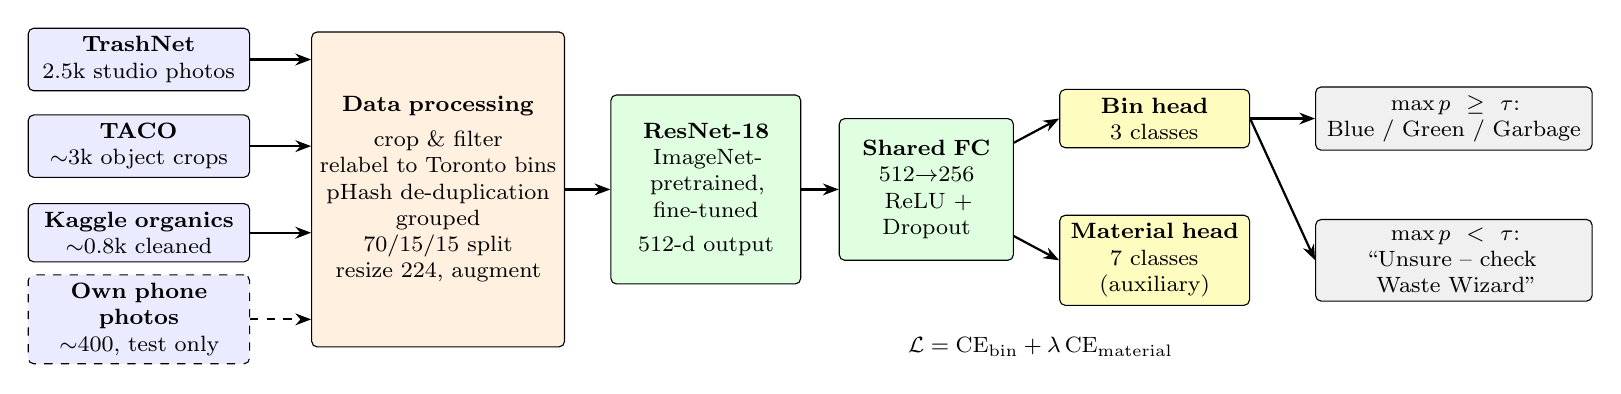
\begin{tikzpicture}[font=\footnotesize,
      box/.style={draw, rounded corners=2pt, align=center, inner sep=3pt},
      arr/.style={-{Stealth[length=2mm]}, thick}]
    \node[box, fill=blue!8, text width=26mm] (d1) at (0,1.65) {\textbf{TrashNet}\\2.5k studio photos};
    \node[box, fill=blue!8, text width=26mm] (d2) at (0,0.55) {\textbf{TACO}\\$\sim$3k object crops};
    \node[box, fill=blue!8, text width=26mm] (d3) at (0,-0.55) {\textbf{Kaggle organics}\\$\sim$0.8k cleaned};
    \node[box, fill=blue!8, dashed, text width=26mm] (d4) at (0,-1.65) {\textbf{Own phone photos}\\$\sim$400, test only};
    \node[box, fill=orange!12, text width=30mm, minimum height=40mm] (p) at (3.8,0) {\textbf{Data processing}\\[3pt] crop \& filter\\ relabel to Toronto bins\\ pHash de-duplication\\ grouped 70/15/15 split\\ resize 224, augment};
    \node[box, fill=green!12, text width=22mm, minimum height=24mm] (b) at (7.2,0) {\textbf{ResNet-18}\\ImageNet-pretrained,\\fine-tuned\\[3pt] 512-d output};
    \node[box, fill=green!12, text width=20mm, minimum height=18mm] (f) at (10.0,0) {\textbf{Shared FC}\\512$\to$256\\ReLU + Dropout};
    \node[box, fill=yellow!25, text width=22mm] (hb) at (12.9,0.9) {\textbf{Bin head}\\3 classes};
    \node[box, fill=yellow!25, text width=22mm] (hm) at (12.9,-0.9) {\textbf{Material head}\\7 classes (auxiliary)};
    \node[box, fill=gray!12, text width=33mm] (o1) at (16.7,0.9) {$\max p \ge \tau$:\\ Blue / Green / Garbage};
    \node[box, fill=gray!12, text width=33mm] (o2) at (16.7,-0.9) {$\max p < \tau$:\\ ``Unsure -- check Waste Wizard''};
    \node[font=\footnotesize] at (11.45,-2.0) {$\mathcal{L} = \mathrm{CE}_{\text{bin}} + \lambda\,\mathrm{CE}_{\text{material}}$};
    \foreach \d in {d1,d2,d3} \draw[arr] (\d.east) -- (\d.east -| p.west);
    \draw[arr, dashed] (d4.east) -- (d4.east -| p.west);
    \draw[arr] (p) -- (b);
    \draw[arr] (b) -- (f);
    \draw[arr] (f) -- (hb.west);
    \draw[arr] (f) -- (hm.west);
    \draw[arr] (hb.east) -- (o1.west);
    \draw[arr] (hb.east) -- (o2.west);
  \end{tikzpicture}}
  \caption{BinSight overview. Four data sources are cleaned and relabelled to Toronto's rules; a pretrained ResNet-18 with two output heads predicts the bin and the material; low-confidence predictions are deferred to the user. Own phone photos are held out for real-world testing.}
  \label{fig:overview}
\end{figure}

\section*{Background \& Related Work}
\textbf{TrashNet}~\cite{thung2016} is a released set of 2,527 photos of single items on a white board in six classes; a SIFT + SVM classifier reached 63\% test accuracy and beat their small CNN. \textbf{RecycleNet}~\cite{bircanoglu2018} compared deep CNNs on TrashNet: fine-tuning an ImageNet-pretrained DenseNet121 gave 95\% accuracy, showing the power of transfer learning, but only on uniform-background images. \textbf{TACO}~\cite{proenca2020} provides 1,500 in-the-wild photos with 4,784 litter instances in 60 categories (COCO format) and a Mask R-CNN baseline, showing how hard cluttered real scenes are. \textbf{Majchrowska et al.}~\cite{majchrowska2022} merged over ten waste datasets into a seven-category benchmark; their EfficientDet-D2 + EfficientNet-B2 system reached only about 75\% classification accuracy, so realistic settings are much harder and label harmonisation across datasets is critical. The \textbf{Kaggle Waste Classification Data}~\cite{sekar2019} has 25,077 web images labelled only organic vs.\ recyclable, and Toronto's \textbf{Waste Wizard}~\cite{wastewizard} is a text lookup, not a visual tool. BinSight differs by predicting \emph{municipal bin rules} rather than generic materials, learning both tasks jointly, abstaining when unsure, and testing on newly collected household photos.

\section*{Data Processing}
\textbf{Sources.} (1) TrashNet~\cite{thung2016}, 2,527 images; (2) TACO~\cite{proenca2020} object crops from \texttt{annotations.json}; (3) the organic class of the Kaggle dataset~\cite{sekar2019}; (4) about 400 phone photos of my own household waste (at least 50 per material class) on varied backgrounds and lighting.
\textbf{Steps.} (a) \emph{TACO cropping:} crop each bounding box with a 10\% margin; drop crops with shorter side under 64\,px and the ``Unlabeled litter'' category ($\sim$3,000 crops expected); keep the source \texttt{image\_id}. (b) \emph{Label harmonisation:} a table \texttt{label\_map.csv} maps every TACO category and TrashNet class to a (material, bin) pair using Waste Wizard look-ups (e.g., \emph{Drink can}$\to$(metal, Blue), \emph{Food waste}$\to$(organic, Green), \emph{Cigarette}$\to$(other, Garbage)); ambiguous categories are dropped and TrashNet's 137 ``trash'' images are relabelled one by one. (c) \emph{Organic cleaning:} sample 1,500 Kaggle organic images and manually remove drawings, collages, text and multi-object scenes (target $\sim$800). (d) \emph{De-duplication:} remove near-duplicates with perceptual hashing (pHash, Hamming distance $\le 4$) before splitting. (e) \emph{Splitting:} 70/15/15 train/validation/test, stratified by bin; all crops of one TACO photo stay in the same split to prevent leakage. Source (4) is never used for training or tuning; it is a separate real-world test set. (f) \emph{Transforms:} pad to square, resize to $224\times224$, normalise with ImageNet statistics; training augmentation uses random resized crop (scale 0.6--1.0), horizontal flip, $\pm15^\circ$ rotation and colour jitter (0.3). Inverse-frequency class weights in the loss handle class imbalance.

\section*{Architecture}
The backbone is \textbf{ResNet-18}~\cite{he2016} pretrained on ImageNet~\cite{deng2009}. Its final layer is replaced by a shared fully-connected layer (512$\to$256, ReLU, dropout 0.3) feeding two linear heads: a 3-way \emph{bin} head and a 7-way \emph{material} head. Training minimises $\mathcal{L}=\mathrm{CE}_{\text{bin}}+\lambda\,\mathrm{CE}_{\text{material}}$ ($\lambda=0.5$, tuned), so the auxiliary task regularises the shared features (multi-task learning~\cite{caruana1997}). Stage 1 freezes the backbone and trains the heads (Adam, lr $10^{-3}$, 5 epochs); stage 2 unfreezes \texttt{layer3}--\texttt{layer4} (lr $10^{-4}$, cosine decay, $\le$30 epochs, batch 64) with early stopping on validation bin macro-F1. If the top bin probability is below a threshold $\tau$, chosen on validation data so that accepted predictions are $\ge$95\% correct, the model abstains~\cite{geifman2017}. Grad-CAM~\cite{selvaraju2017} checks that the model looks at the item, not the background; ablations compare single- vs.\ multi-task and frozen vs.\ fine-tuned backbones.
\textbf{Success criteria:} bin accuracy $\ge$85\% on the test split and $\ge$75\% on my own photos, at least 15 points above the baseline, also reporting macro-F1, confusion matrices and coverage (share of non-abstained predictions).

\section*{Baseline Model}
Both baselines use exactly the same splits. (1) A \emph{majority-class} predictor gives a lower bound. (2) A classical pipeline: resize to $128\times128$; extract HOG features~\cite{dalal2005} from the grayscale image (9 orientations, $16\times16$\,px cells, $2\times2$-cell blocks, 1,764-d) and an HSV colour histogram ($8\times8\times8=512$-d); concatenate, standardise, reduce to 256-d with PCA and train RBF-kernel SVMs~\cite{cortes1995} for bin and material (grid search $C\in\{0.1,1,10,100\}$, $\gamma\in\{10^{-4},10^{-3},10^{-2}\}$ on validation) using scikit-image and scikit-learn. This mirrors TrashNet's SIFT + SVM approach~\cite{thung2016}.

\section*{Ethical Considerations}
\emph{Data:} TACO images come from Flickr and may show people or plates; I use object crops only and drop any crop with a person. TACO annotations are CC BY 4.0 and the Kaggle set is CC BY-SA 4.0; all sources are credited. My own photos exclude addresses and have EXIF removed. \emph{Bias and limits:} training images are mostly from the US, Europe and the web, so Canadian packaging may be under-represented. Bin rules are municipal and change over time, so predictions are not valid outside Toronto and the mapping table is versioned. \emph{Impact of errors:} a wrong Blue Bin answer adds contamination, and hazardous items such as lithium batteries are out of scope. The model abstains when unsure, points users to Waste Wizard, and is not for monitoring residents.

\newpage
\bibliographystyle{plain}
\bibliography{references}

\end{document}
